% Options for packages loaded elsewhere
\PassOptionsToPackage{unicode}{hyperref}
\PassOptionsToPackage{hyphens}{url}
%
\documentclass[
]{article}
\usepackage{amsmath,amssymb}
\usepackage{lmodern}
\usepackage{iftex}
\ifPDFTeX
  \usepackage[T1]{fontenc}
  \usepackage[utf8]{inputenc}
  \usepackage{textcomp} % provide euro and other symbols
\else % if luatex or xetex
  \usepackage{unicode-math}
  \defaultfontfeatures{Scale=MatchLowercase}
  \defaultfontfeatures[\rmfamily]{Ligatures=TeX,Scale=1}
\fi
% Use upquote if available, for straight quotes in verbatim environments
\IfFileExists{upquote.sty}{\usepackage{upquote}}{}
\IfFileExists{microtype.sty}{% use microtype if available
  \usepackage[]{microtype}
  \UseMicrotypeSet[protrusion]{basicmath} % disable protrusion for tt fonts
}{}
\makeatletter
\@ifundefined{KOMAClassName}{% if non-KOMA class
  \IfFileExists{parskip.sty}{%
    \usepackage{parskip}
  }{% else
    \setlength{\parindent}{0pt}
    \setlength{\parskip}{6pt plus 2pt minus 1pt}}
}{% if KOMA class
  \KOMAoptions{parskip=half}}
\makeatother
\usepackage{xcolor}
\usepackage[margin=1in]{geometry}
\usepackage{color}
\usepackage{fancyvrb}
\newcommand{\VerbBar}{|}
\newcommand{\VERB}{\Verb[commandchars=\\\{\}]}
\DefineVerbatimEnvironment{Highlighting}{Verbatim}{commandchars=\\\{\}}
% Add ',fontsize=\small' for more characters per line
\usepackage{framed}
\definecolor{shadecolor}{RGB}{248,248,248}
\newenvironment{Shaded}{\begin{snugshade}}{\end{snugshade}}
\newcommand{\AlertTok}[1]{\textcolor[rgb]{0.94,0.16,0.16}{#1}}
\newcommand{\AnnotationTok}[1]{\textcolor[rgb]{0.56,0.35,0.01}{\textbf{\textit{#1}}}}
\newcommand{\AttributeTok}[1]{\textcolor[rgb]{0.77,0.63,0.00}{#1}}
\newcommand{\BaseNTok}[1]{\textcolor[rgb]{0.00,0.00,0.81}{#1}}
\newcommand{\BuiltInTok}[1]{#1}
\newcommand{\CharTok}[1]{\textcolor[rgb]{0.31,0.60,0.02}{#1}}
\newcommand{\CommentTok}[1]{\textcolor[rgb]{0.56,0.35,0.01}{\textit{#1}}}
\newcommand{\CommentVarTok}[1]{\textcolor[rgb]{0.56,0.35,0.01}{\textbf{\textit{#1}}}}
\newcommand{\ConstantTok}[1]{\textcolor[rgb]{0.00,0.00,0.00}{#1}}
\newcommand{\ControlFlowTok}[1]{\textcolor[rgb]{0.13,0.29,0.53}{\textbf{#1}}}
\newcommand{\DataTypeTok}[1]{\textcolor[rgb]{0.13,0.29,0.53}{#1}}
\newcommand{\DecValTok}[1]{\textcolor[rgb]{0.00,0.00,0.81}{#1}}
\newcommand{\DocumentationTok}[1]{\textcolor[rgb]{0.56,0.35,0.01}{\textbf{\textit{#1}}}}
\newcommand{\ErrorTok}[1]{\textcolor[rgb]{0.64,0.00,0.00}{\textbf{#1}}}
\newcommand{\ExtensionTok}[1]{#1}
\newcommand{\FloatTok}[1]{\textcolor[rgb]{0.00,0.00,0.81}{#1}}
\newcommand{\FunctionTok}[1]{\textcolor[rgb]{0.00,0.00,0.00}{#1}}
\newcommand{\ImportTok}[1]{#1}
\newcommand{\InformationTok}[1]{\textcolor[rgb]{0.56,0.35,0.01}{\textbf{\textit{#1}}}}
\newcommand{\KeywordTok}[1]{\textcolor[rgb]{0.13,0.29,0.53}{\textbf{#1}}}
\newcommand{\NormalTok}[1]{#1}
\newcommand{\OperatorTok}[1]{\textcolor[rgb]{0.81,0.36,0.00}{\textbf{#1}}}
\newcommand{\OtherTok}[1]{\textcolor[rgb]{0.56,0.35,0.01}{#1}}
\newcommand{\PreprocessorTok}[1]{\textcolor[rgb]{0.56,0.35,0.01}{\textit{#1}}}
\newcommand{\RegionMarkerTok}[1]{#1}
\newcommand{\SpecialCharTok}[1]{\textcolor[rgb]{0.00,0.00,0.00}{#1}}
\newcommand{\SpecialStringTok}[1]{\textcolor[rgb]{0.31,0.60,0.02}{#1}}
\newcommand{\StringTok}[1]{\textcolor[rgb]{0.31,0.60,0.02}{#1}}
\newcommand{\VariableTok}[1]{\textcolor[rgb]{0.00,0.00,0.00}{#1}}
\newcommand{\VerbatimStringTok}[1]{\textcolor[rgb]{0.31,0.60,0.02}{#1}}
\newcommand{\WarningTok}[1]{\textcolor[rgb]{0.56,0.35,0.01}{\textbf{\textit{#1}}}}
\usepackage{graphicx}
\makeatletter
\def\maxwidth{\ifdim\Gin@nat@width>\linewidth\linewidth\else\Gin@nat@width\fi}
\def\maxheight{\ifdim\Gin@nat@height>\textheight\textheight\else\Gin@nat@height\fi}
\makeatother
% Scale images if necessary, so that they will not overflow the page
% margins by default, and it is still possible to overwrite the defaults
% using explicit options in \includegraphics[width, height, ...]{}
\setkeys{Gin}{width=\maxwidth,height=\maxheight,keepaspectratio}
% Set default figure placement to htbp
\makeatletter
\def\fps@figure{htbp}
\makeatother
\setlength{\emergencystretch}{3em} % prevent overfull lines
\providecommand{\tightlist}{%
  \setlength{\itemsep}{0pt}\setlength{\parskip}{0pt}}
\setcounter{secnumdepth}{-\maxdimen} % remove section numbering
\usepackage{booktabs}
\usepackage{longtable}
\usepackage{array}
\usepackage{multirow}
\usepackage{wrapfig}
\usepackage{float}
\usepackage{colortbl}
\usepackage{pdflscape}
\usepackage{tabu}
\usepackage{threeparttable}
\usepackage{threeparttablex}
\usepackage[normalem]{ulem}
\usepackage{makecell}
\usepackage{xcolor}
\ifLuaTeX
  \usepackage{selnolig}  % disable illegal ligatures
\fi
\IfFileExists{bookmark.sty}{\usepackage{bookmark}}{\usepackage{hyperref}}
\IfFileExists{xurl.sty}{\usepackage{xurl}}{} % add URL line breaks if available
\urlstyle{same} % disable monospaced font for URLs
\hypersetup{
  pdftitle={Siwa PETS},
  hidelinks,
  pdfcreator={LaTeX via pandoc}}

\title{Siwa PETS}
\author{}
\date{\vspace{-2.5em}}

\begin{document}
\maketitle

\begin{verbatim}
## 
## Attaching package: 'shinydashboard'
\end{verbatim}

\begin{verbatim}
## The following object is masked from 'package:graphics':
## 
##     box
\end{verbatim}

\begin{verbatim}
## Loading required package: usethis
\end{verbatim}

\begin{verbatim}
## 
## Attaching package: 'flexdashboard'
\end{verbatim}

\begin{verbatim}
## The following objects are masked from 'package:shinydashboard':
## 
##     renderValueBox, valueBox, valueBoxOutput
\end{verbatim}

\begin{verbatim}
## Warning in !is.null(rmarkdown::metadata$output) && rmarkdown::metadata$output
## %in% : 'length(x) = 2 > 1' in coercion to 'logical(1)'
\end{verbatim}

\begin{verbatim}
## 
## microbiome R package (microbiome.github.com)
##     
## 
## 
##  Copyright (C) 2011-2022 Leo Lahti, 
##     Sudarshan Shetty et al. <microbiome.github.io>
\end{verbatim}

\begin{verbatim}
## 
## Attaching package: 'microbiome'
\end{verbatim}

\begin{verbatim}
## The following object is masked from 'package:ggplot2':
## 
##     alpha
\end{verbatim}

\begin{verbatim}
## The following object is masked from 'package:base':
## 
##     transform
\end{verbatim}

\begin{verbatim}
## 
## Attaching package: 'plotly'
\end{verbatim}

\begin{verbatim}
## The following objects are masked from 'package:plyr':
## 
##     arrange, mutate, rename, summarise
\end{verbatim}

\begin{verbatim}
## The following object is masked from 'package:ggplot2':
## 
##     last_plot
\end{verbatim}

\begin{verbatim}
## The following object is masked from 'package:stats':
## 
##     filter
\end{verbatim}

\begin{verbatim}
## The following object is masked from 'package:graphics':
## 
##     layout
\end{verbatim}

\begin{verbatim}
## Loading required package: dplyr
\end{verbatim}

\begin{verbatim}
## 
## Attaching package: 'dplyr'
\end{verbatim}

\begin{verbatim}
## The following objects are masked from 'package:plyr':
## 
##     arrange, count, desc, failwith, id, mutate, rename, summarise,
##     summarize
\end{verbatim}

\begin{verbatim}
## The following object is masked from 'package:kableExtra':
## 
##     group_rows
\end{verbatim}

\begin{verbatim}
## The following objects are masked from 'package:stats':
## 
##     filter, lag
\end{verbatim}

\begin{verbatim}
## The following objects are masked from 'package:base':
## 
##     intersect, setdiff, setequal, union
\end{verbatim}

\begin{verbatim}
## Warning: replacing previous import 'ggplot2::alpha' by 'microbiome::alpha' when
## loading 'microbiomeutilities'
\end{verbatim}

\begin{verbatim}
## 
## Attaching package: 'microbiomeutilities'
\end{verbatim}

\begin{verbatim}
## The following object is masked from 'package:microbiome':
## 
##     add_refseq
\end{verbatim}

\begin{verbatim}
## microViz version 0.10.8 - Copyright (C) 2022 David Barnett
## Attaching package: 'microViz'
## The following object is masked from 'package:plotly':
## 
## add_paths
## Loading required package: tidyverse
## -- Attaching core tidyverse packages ------------------------ tidyverse 2.0.0
## -- v forcats 1.0.0 v readr 2.1.4 v lubridate 1.9.2 v tibble 3.2.0 v purrr 1.0.1
## v tidyr 1.3.0
## -- Conflicts ------------------------------------------ tidyverse_conflicts()
## -- x microbiome::alpha() masks ggplot2::alpha() x dplyr::arrange() masks
## plotly::arrange(), plyr::arrange() x purrr::compact() masks plyr::compact() x
## dplyr::count() masks plyr::count() x dplyr::desc() masks plyr::desc() x
## dplyr::failwith() masks plyr::failwith() x dplyr::filter() masks
## plotly::filter(), stats::filter() x dplyr::group_rows() masks
## kableExtra::group_rows() x dplyr::id() masks plyr::id() x dplyr::lag() masks
## stats::lag() x dplyr::mutate() masks plotly::mutate(), plyr::mutate() x
## dplyr::rename() masks plotly::rename(), plyr::rename() x dplyr::summarise()
## masks plotly::summarise(), plyr::summarise() x dplyr::summarize() masks
## plyr::summarize() i Use the ]8;;http://conflicted.r-lib.org/conflicted package]8;; to force all conflicts to become
## errors
## Attaching package: 'tidyMicro'
## The following object is masked from 'package:microViz':
## 
## cor_heatmap
## The following object is masked from 'package:microbiomeutilities':
## 
## taxa_summary
## ! Website: https://david-barnett.github.io/microViz
## v Useful?  For citation details, run: `citation("microViz")`
## x Silence? `suppressPackageStartupMessages(library(microViz))`
\end{verbatim}

\hypertarget{project-description}{%
\section{Project description}\label{project-description}}

\hypertarget{row}{%
\subsection{Row}\label{row}}

\hypertarget{section}{%
\subsubsection{}\label{section}}

\begin{Shaded}
\begin{Highlighting}[]
\NormalTok{knitr}\SpecialCharTok{::}\FunctionTok{include\_graphics}\NormalTok{(}\StringTok{"perro.jpg"}\NormalTok{)}
\end{Highlighting}
\end{Shaded}

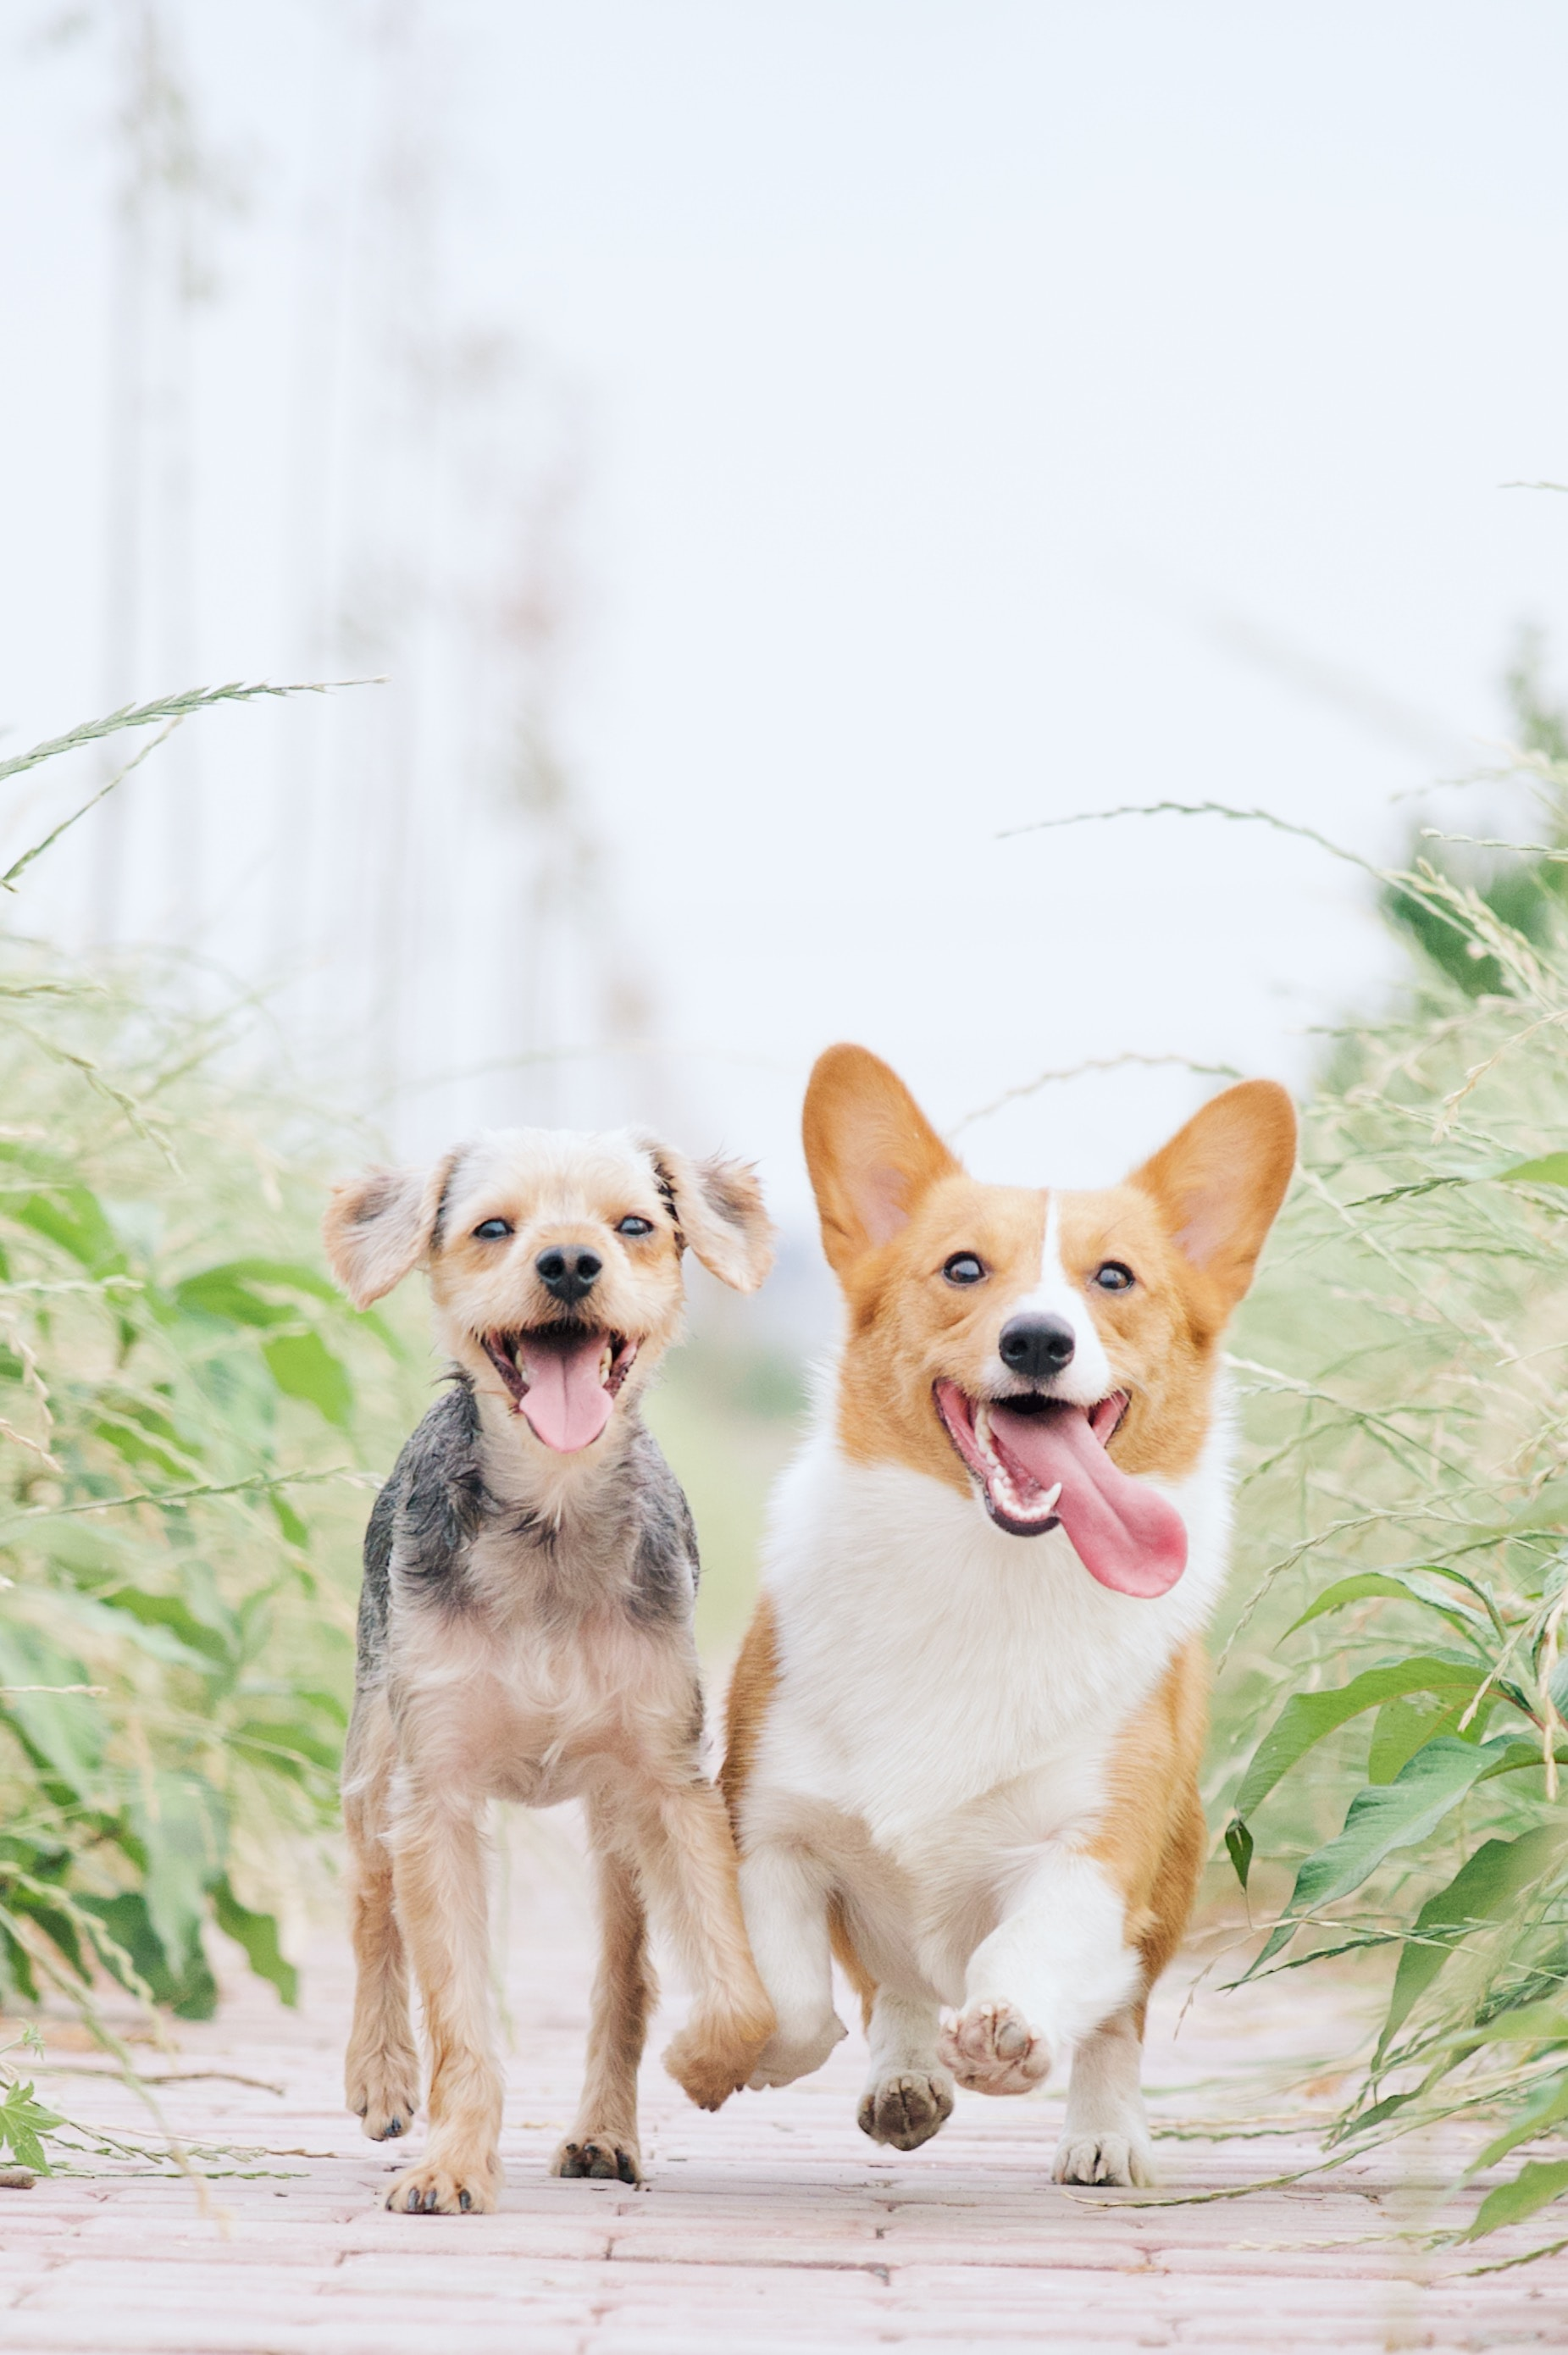
\includegraphics[width=25.71in]{perro}

\begin{Shaded}
\begin{Highlighting}[]
\NormalTok{cvi\_colours }\OtherTok{=} \FunctionTok{list}\NormalTok{(}
  \AttributeTok{cvi\_siwa =} \FunctionTok{c}\NormalTok{(}\StringTok{"\#03343a"}\NormalTok{, }\StringTok{"\#4e8e74"}\NormalTok{,}\StringTok{"\#f99b35"}\NormalTok{,  }\StringTok{"\#e5c217"}\NormalTok{,  }
               \StringTok{"\#075b44"}\NormalTok{, }\StringTok{"\#f9b870"}\NormalTok{, }\StringTok{"\#f7e76d"}\NormalTok{, }
                  \StringTok{"\#017fb1"}\NormalTok{, }\StringTok{"\#5cb08e"}\NormalTok{ , }\StringTok{"\#fcd8b6"}\NormalTok{, }\StringTok{"\#fcf5cd"}\NormalTok{, }\StringTok{"\#ABF4D4"}\NormalTok{,}
               \StringTok{"\#8CDBF4"}\NormalTok{,}\StringTok{"\#F7927F"}\NormalTok{),}
  
  \AttributeTok{alpha\_colors =} \FunctionTok{c}\NormalTok{( }\StringTok{"\#075b44"}\NormalTok{,  }\StringTok{"\#017fb1"}\NormalTok{),}
  \AttributeTok{bad\_good\_stool =} \FunctionTok{c}\NormalTok{( }\StringTok{"\#f9b870"}\NormalTok{,}\StringTok{"\#f9b870"}\NormalTok{, }\StringTok{"\#5cb08e"}\NormalTok{),}
  \AttributeTok{groups\_pastel =} \FunctionTok{c}\NormalTok{( ), }
  \AttributeTok{groups=}\FunctionTok{c}\NormalTok{(}\StringTok{"\#4e8e74"}\NormalTok{, }\StringTok{"\#035060"}\NormalTok{, }\StringTok{"\#f99b35"}\NormalTok{, }\StringTok{"\#BC8808"}\NormalTok{)}
\NormalTok{)}

\NormalTok{cvi\_palettes }\OtherTok{=} \ControlFlowTok{function}\NormalTok{(name, n, }\AttributeTok{all\_palettes =}\NormalTok{ cvi\_colours, }\AttributeTok{type =} \FunctionTok{c}\NormalTok{(}\StringTok{"discrete"}\NormalTok{, }\StringTok{"continuous"}\NormalTok{)) \{}
\NormalTok{  palette }\OtherTok{=}\NormalTok{ all\_palettes[[name]]}
  \ControlFlowTok{if}\NormalTok{ (}\FunctionTok{missing}\NormalTok{(n)) \{}
\NormalTok{    n }\OtherTok{=} \FunctionTok{length}\NormalTok{(palette)}
\NormalTok{  \}}
\NormalTok{  type }\OtherTok{=} \FunctionTok{match.arg}\NormalTok{(type)}
\NormalTok{  out }\OtherTok{=} \ControlFlowTok{switch}\NormalTok{(type,}\AttributeTok{continuous =}\NormalTok{ grDevices}\SpecialCharTok{::}\FunctionTok{colorRampPalette}\NormalTok{(palette)(n),}\AttributeTok{discrete =}\NormalTok{ palette[}\DecValTok{1}\SpecialCharTok{:}\NormalTok{n]}
\NormalTok{  )}
  \FunctionTok{structure}\NormalTok{(out, }\AttributeTok{name =}\NormalTok{ name, }\AttributeTok{class =} \StringTok{"palette"}\NormalTok{)}
\NormalTok{\}}

\NormalTok{scale\_color\_cvi\_d }\OtherTok{=} \ControlFlowTok{function}\NormalTok{(name) \{}
\NormalTok{  ggplot2}\SpecialCharTok{::}\FunctionTok{scale\_colour\_manual}\NormalTok{(}\AttributeTok{values =} \FunctionTok{cvi\_palettes}\NormalTok{(name, }\AttributeTok{type =} \StringTok{"discrete"}\NormalTok{))}
\NormalTok{\}}
\NormalTok{scale\_fill\_cvi\_d }\OtherTok{=} \ControlFlowTok{function}\NormalTok{(name) \{}
\NormalTok{  ggplot2}\SpecialCharTok{::}\FunctionTok{scale\_fill\_manual}\NormalTok{(}\AttributeTok{values =} \FunctionTok{cvi\_palettes}\NormalTok{(name,}\AttributeTok{type =} \StringTok{"discrete"}\NormalTok{))}
\NormalTok{\}}
\end{Highlighting}
\end{Shaded}

\hypertarget{section-1}{%
\subsubsection{}\label{section-1}}

\textbf{NAME OF THE EXPERIMENT !!! }

Lorem Ipsum is simply dummy text of the printing and typesetting
industry. Lorem Ipsum has been the industry's standard dummy text ever
since the 1500s, when an unknown printer took a galley of type and
scrambled it to make a type specimen book. It has survived not only five
centuries, but also the leap into electronic typesetting, remaining
essentially unchanged. It was popularised in the 1960s with the release
of Letraset sheets containing Lorem Ipsum passages, and more recently
with desktop publishing software like Aldus PageMaker including versions
of Lorem Ipsum.

\hypertarget{microbiome-composition}{%
\section{Microbiome composition}\label{microbiome-composition}}

\hypertarget{row-1}{%
\subsection{Row}\label{row-1}}

Lorem ipsum dolor sit amet, consectetur adipiscing elit, sed do eiusmod
tempor incididunt ut labore et dolore magna aliqua. Ut enim ad minim
veniam, quis nostrud exercitation ullamco laboris nisi ut aliquip ex ea
commodo consequat. Duis aute irure dolor in reprehenderit in voluptate
velit esse cillum dolore eu fugiat nulla pariatur. Excepteur sint
occaecat cupidatat non proident, sunt in culpa qui officia deserunt
mollit anim id est laborum

\hypertarget{row-2}{%
\subsection{Row}\label{row-2}}

\hypertarget{row-3}{%
\subsection{Row}\label{row-3}}

\hypertarget{beta-diversity-timepoint-after}{%
\subsubsection{Beta diversity: timepoint
after}\label{beta-diversity-timepoint-after}}

\begin{Shaded}
\begin{Highlighting}[]
\NormalTok{out.bray }\OtherTok{\textless{}{-}}
    \FunctionTok{ordinate}\NormalTok{(}
\NormalTok{      phylo\_after, }\AttributeTok{method =} \StringTok{"MDS"}\NormalTok{, }
      \AttributeTok{distance =} \StringTok{"bray"}\NormalTok{)}
\NormalTok{p }\OtherTok{\textless{}{-}} \FunctionTok{plot\_ordination}\NormalTok{(}
\NormalTok{    phylo\_after,}
\NormalTok{    out.bray,}
    \AttributeTok{color =} \StringTok{"Group"}\NormalTok{,}
    \AttributeTok{axes =} \FunctionTok{c}\NormalTok{(}\DecValTok{1}\NormalTok{, }\DecValTok{2}\NormalTok{),}
    \AttributeTok{justDF =} \ConstantTok{FALSE}
\NormalTok{  )}
\NormalTok{df }\OtherTok{\textless{}{-}}\NormalTok{ p}\SpecialCharTok{$}\NormalTok{data}
\NormalTok{df}\SpecialCharTok{$}\NormalTok{Group }\OtherTok{\textless{}{-}} \FunctionTok{as.factor}\NormalTok{(df}\SpecialCharTok{$}\NormalTok{Group)}
\NormalTok{plot }\OtherTok{\textless{}{-}} \FunctionTok{ggplot}\NormalTok{(df, }\FunctionTok{aes}\NormalTok{(}
    \AttributeTok{x =}\NormalTok{ Axis}\FloatTok{.1}\NormalTok{,}
    \AttributeTok{y =}\NormalTok{ Axis}\FloatTok{.2}\NormalTok{,}
    \AttributeTok{color =}\NormalTok{ Group,}
    \AttributeTok{text =} \FunctionTok{paste}\NormalTok{(}\StringTok{"Dog:"}\NormalTok{, DOG, }\StringTok{"}\SpecialCharTok{\textbackslash{}n}\StringTok{"}\NormalTok{, DogGroup) )) }\SpecialCharTok{+}
    \FunctionTok{geom\_point}\NormalTok{(}\AttributeTok{size=}\DecValTok{3}\NormalTok{) }\SpecialCharTok{+} \FunctionTok{scale\_color\_cvi\_d}\NormalTok{(}\StringTok{"groups"}\NormalTok{) }\SpecialCharTok{+}\FunctionTok{xlab}\NormalTok{(p}\SpecialCharTok{$}\NormalTok{labels}\SpecialCharTok{$}\NormalTok{x) }\SpecialCharTok{+} \FunctionTok{ylab}\NormalTok{(p}\SpecialCharTok{$}\NormalTok{labels}\SpecialCharTok{$}\NormalTok{y)}

\NormalTok{plot}
\end{Highlighting}
\end{Shaded}

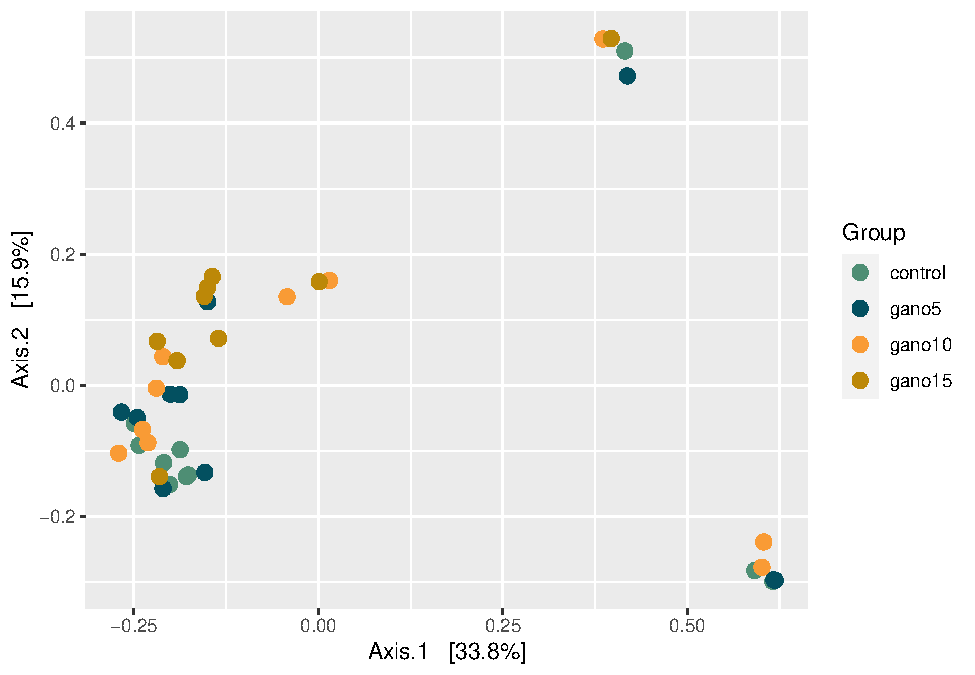
\includegraphics{pets_public_files/figure-latex/beta-1.pdf}

\begin{Shaded}
\begin{Highlighting}[]
\CommentTok{\#ggplotly(plot, tooltip = "text", height = 500)}
\end{Highlighting}
\end{Shaded}

\hypertarget{row-4}{%
\subsection{Row}\label{row-4}}

\end{document}
